% =============================================================================
% Section 4: Axis Diagnostics
% =============================================================================
\section{Axis-Level Diagnostics}\label{sec:axis-diagnostics}

This section examines the distributional properties of each axis,
identifies axis dominance patterns, decomposes the cross-country
composite variance into axis-level contributions with a formal proof,
quantifies each axis's contribution to rank differentiation, and
provides a structural analysis of the defence axis.

\subsection{Axis summary statistics}

\Cref{tab:axis-stats} reports distributional statistics for each of
the six axes.  The coefficient of variation (CV = $\sigma / \mu$)
provides a scale-free measure of relative dispersion.

\begin{table}[htbp]
\centering
\caption{Axis-level distributional statistics, EU-27, 2024.}
\label{tab:axis-stats}
\begin{tabular}{@{}lS[table-format=1.8]S[table-format=1.8]
  S[table-format=1.8]S[table-format=1.8]S[table-format=1.8]
  S[table-format=1.4]@{}}
\toprule
{\textbf{Axis}} & {\textbf{Min}} & {\textbf{Max}} & {\textbf{Mean}}
  & {\textbf{Median}} & {$\boldsymbol{\sigma}$ \textbf{(pop.)}}
  & {\textbf{CV}} \\
\midrule
Financial       & 0.10039135 & 0.27299265 & 0.14799792 & 0.13998786 & 0.03728203 & 0.2519 \\
Energy          & 0.30187479 & 0.47029821 & 0.36523663 & 0.35125471 & 0.04790658 & 0.1312 \\
Technology      & 0.09762824 & 0.58695939 & 0.21078775 & 0.19789321 & 0.09458972 & 0.4488 \\
Defence         & 0.00000000 & 1.00000000 & 0.57319930 & 0.55148593 & 0.22565797 & 0.3936 \\
Critical inputs & 0.11235234 & 0.54699996 & 0.25154982 & 0.22200621 & 0.12182538 & 0.4843 \\
Logistics       & 0.27295297 & 1.00000000 & 0.51757723 & 0.47781001 & 0.18640808 & 0.3603 \\
\bottomrule
\end{tabular}
\end{table}

Several patterns are noteworthy:

\begin{itemize}[leftmargin=2em]
  \item \textbf{Highest dispersion.}  Critical inputs has the highest
    CV (0.4843), followed by technology (0.4488).  These axes
    contribute the most relative cross-country differentiation per
    unit of mean score.

  \item \textbf{Lowest dispersion.}  Energy has the lowest CV
    (0.1312) and the smallest range (\num{0.16842342}), indicating
    that EU countries exhibit comparatively homogeneous energy
    dependency concentration.

  \item \textbf{Highest absolute dispersion.}  Defence has the
    largest population standard deviation (\num{0.22565797}) and
    the largest range (1.0), spanning the entire unit interval from
    Slovakia's \num{0.00000000} to Malta's \num{1.00000000}.

  \item \textbf{Lowest mean.}  The financial axis has the lowest mean
    (\num{0.14799792}).  All 27~countries score below 0.28 on this
    axis, indicating dispersed counterparty structures in cross-border
    financial exposures.

  \item \textbf{Highest means.}  Defence (\num{0.57319930}) and
    logistics (\num{0.51757723}) record the highest axis means.
    These axes pull the composite upward on average.
\end{itemize}

The contrast between relative and absolute dispersion is
consequential for the variance decomposition below.  The financial
axis has moderate relative dispersion (CV = 0.252) but very low
absolute dispersion ($\sigma = 0.037$).  Because the composite is an
unweighted arithmetic mean, it is the \emph{absolute} dispersion that
determines variance contribution.  This explains why the financial
axis contributes negligibly to composite variance despite having
non-trivial relative variation.

\subsection{Axis distributions: boxplots}

\Cref{fig:boxplots} displays boxplots for all six axes, permitting
direct visual comparison of location, spread, and skewness.

\begin{figure}[htbp]
\centering
% F04: Boxplots of the six ISI axes
\begin{tikzpicture}
\begin{axis}[
  width=0.90\textwidth,
  height=0.50\textwidth,
  boxplot/draw direction=y,
  ylabel={Axis score},
  ymin=-0.05, ymax=1.10,
  xtick={1,2,3,4,5,6},
  xticklabels={Financial, Energy, Technology, Defence, Crit.~Inputs, Logistics},
  x tick label style={font=\small, rotate=25, anchor=east},
  tick label style={font=\small},
  label style={font=\small},
  grid=major,
  grid style={gray!30},
]
% Financial: Q1=0.1217 Med=0.1400 Q3=0.1614 Lo=0.1004 Hi=0.2008 Out_hi=1 (0.2730)
\addplot+[boxplot prepared={
  lower whisker=0.1004,
  lower quartile=0.1217,
  median=0.1400,
  upper quartile=0.1614,
  upper whisker=0.2008},
  fill=blue!20, draw=blue!60
] coordinates {(1,0.2730)};

% Energy: Q1=0.3320 Med=0.3513 Q3=0.3929 Lo=0.3019 Hi=0.4703 Out=0
\addplot+[boxplot prepared={
  lower whisker=0.3019,
  lower quartile=0.3320,
  median=0.3513,
  upper quartile=0.3929,
  upper whisker=0.4703},
  fill=green!20, draw=green!60
] coordinates {};

% Technology: Q1=0.1510 Med=0.1979 Q3=0.2263 Lo=0.0976 Hi=0.2969 Out_hi=2 (0.3574, 0.5870)
\addplot+[boxplot prepared={
  lower whisker=0.0976,
  lower quartile=0.1510,
  median=0.1979,
  upper quartile=0.2263,
  upper whisker=0.2969},
  fill=orange!20, draw=orange!60
] coordinates {(3,0.3574) (3,0.5870)};

% Defence: Q1=0.4180 Med=0.5515 Q3=0.7351 Lo=0.0000 Hi=1.0000 Out=0
\addplot+[boxplot prepared={
  lower whisker=0.0000,
  lower quartile=0.4180,
  median=0.5515,
  upper quartile=0.7351,
  upper whisker=1.0000},
  fill=red!20, draw=red!60
] coordinates {};

% Critical Inputs: Q1=0.1597 Med=0.2220 Q3=0.3129 Lo=0.1124 Hi=0.5239 Out_hi=1 (0.5470)
\addplot+[boxplot prepared={
  lower whisker=0.1124,
  lower quartile=0.1597,
  median=0.2220,
  upper quartile=0.3129,
  upper whisker=0.5239},
  fill=purple!20, draw=purple!60
] coordinates {(5,0.5470)};

% Logistics: Q1=0.3604 Med=0.4778 Q3=0.6162 Lo=0.2730 Hi=0.9411 Out_hi=1 (1.0000)
\addplot+[boxplot prepared={
  lower whisker=0.2730,
  lower quartile=0.3604,
  median=0.4778,
  upper quartile=0.6162,
  upper whisker=0.9411},
  fill=cyan!20, draw=cyan!60
] coordinates {(6,1.0000)};

\end{axis}
\end{tikzpicture}

\caption{Boxplots of axis-level scores, EU-27, 2024.  The box spans
  Q1--Q3; the line is the median; whiskers extend to the most extreme
  observation within $1.5 \times \text{IQR}$ of the box; circles mark
  outliers beyond the whiskers.}
\label{fig:boxplots}
\end{figure}

\subsection{Top-5 and bottom-5 by axis}

\Cref{tab:axis-top-bottom} lists the five most concentrated and five
least concentrated countries on each axis.  This complements the
composite ranking by revealing axis-specific concentration patterns
that the scalar composite necessarily obscures.

% Table T6: Top-5 and Bottom-5 per axis
\begin{table}[htbp]
\centering
\caption{Top-5 (most concentrated) and Bottom-5 (least concentrated) countries per axis.}
\label{tab:axis-top-bottom}
\small
\setlength{\tabcolsep}{4pt}
\begin{tabular*}{\textwidth}{@{\extracolsep{\fill}} l l S[table-format=1.4] l S[table-format=1.4] @{}}
\toprule
{\textbf{Axis}} & {\textbf{Top-5 (most)}} & {\textbf{Score}} & {\textbf{Bot-5 (least)}} & {\textbf{Score}} \\
\midrule
  Financial & Croatia & 0.2729 & France & 0.1003 \\
   & Greece & 0.2007 & Germany & 0.1018 \\
   & Romania & 0.2003 & Luxembourg & 0.1146 \\
   & Italy & 0.1875 & Sweden & 0.1164 \\
   & Portugal & 0.1830 & Finland & 0.1177 \\
\addlinespace
  Energy & Denmark & 0.4702 & Spain & 0.3018 \\
   & Ireland & 0.4647 & Italy & 0.3078 \\
   & Austria & 0.4558 & Belgium & 0.3078 \\
   & Estonia & 0.4393 & France & 0.3091 \\
   & Romania & 0.4054 & Netherlands & 0.3199 \\
\addlinespace
  Technology & Ireland & 0.5869 & Germany & 0.0976 \\
   & Slovenia & 0.3573 & Sweden & 0.1198 \\
   & Romania & 0.2969 & France & 0.1200 \\
   & Belgium & 0.2945 & Netherlands & 0.1252 \\
   & Austria & 0.2605 & Latvia & 0.1330 \\
\addlinespace
  Defence & Malta & 1.0000 & Slovakia & 0.0000 \\
   & Netherlands & 0.9595 & Latvia & 0.3407 \\
   & Italy & 0.9205 & Estonia & 0.3556 \\
   & Sweden & 0.8810 & France & 0.3703 \\
   & Bulgaria & 0.8606 & Spain & 0.3808 \\
\addlinespace
  Crit.\ Inputs & Finland & 0.5469 & Spain & 0.1123 \\
   & Croatia & 0.5239 & Netherlands & 0.1301 \\
   & Denmark & 0.4362 & Lithuania & 0.1305 \\
   & Cyprus & 0.4235 & Bulgaria & 0.1484 \\
   & Malta & 0.4087 & Latvia & 0.1512 \\
\addlinespace
  Logistics & Malta & 1.0000 & Germany & 0.2729 \\
   & Cyprus & 0.9410 & Romania & 0.2874 \\
   & Finland & 0.7973 & Lithuania & 0.3468 \\
   & Sweden & 0.7551 & Belgium & 0.3520 \\
   & Greece & 0.7198 & France & 0.3529 \\
\bottomrule
\end{tabular*}
\end{table}


Several axis-specific patterns warrant comment.  On the financial
axis, Croatia records the highest score (0.273), which is still
substantially below the median on defence or logistics.  On the
technology axis, Ireland is a clear outlier (0.587), nearly double
the second-highest (Slovenia, 0.357).  On critical inputs, Finland
(0.547) and Croatia (0.524) lead, both small open economies with
concentrated mineral-import partnerships.

\subsection{Axis dominance}\label{sec:axis-dominance}

For each country, we identify the axis with the highest score (``max
axis'') and the axis with the second-highest score.
\Cref{tab:axis-dominance-summary} summarises the count of countries
for which each axis is the maximum.

\begin{table}[htbp]
\centering
\caption{Axis dominance: number of countries for which each axis
  records the highest score.}
\label{tab:axis-dominance-summary}
\begin{tabular}{@{}lr@{}}
\toprule
\textbf{Axis} & \textbf{Count (max axis)} \\
\midrule
Financial       & 0 \\
Energy          & 0 \\
Technology      & 0 \\
Defence         & 16 \\
Critical inputs & 0 \\
Logistics       & 11 \\
\midrule
Total           & 27 \\
\bottomrule
\end{tabular}
\end{table}

The axis-dominance distribution is strikingly concentrated: only two
of six axes ever hold the maximum position.  Defence is the dominant
axis for 16~countries (59.3\%) and logistics for 11~countries (40.7\%).
No country has its highest score on the financial, energy, technology,
or critical-inputs axis.  This implies that for every EU-27 country,
either defence or logistics is the most concentrated domain.

This dominance pattern is not merely a consequence of higher means.
The defence axis mean (0.573) and logistics axis mean (0.518) are
indeed the highest, but several countries have technology or
critical-inputs scores that approach or exceed their defence/logistics
scores.  The dominance concentration reflects a genuine structural
feature: defence and logistics markets in Europe are intrinsically
oligopsonistic, with small buyers facing few feasible suppliers.

The full country-level axis-dominance table, including the max and
second-max axis for each country, is provided in \cref{tab:axis-dominance}
(\cref{app:tables}).

\Cref{fig:axis-dominance-bar} provides a bar-chart visualisation.

\begin{figure}[htbp]
\centering
% F07: Axis dominance bar chart
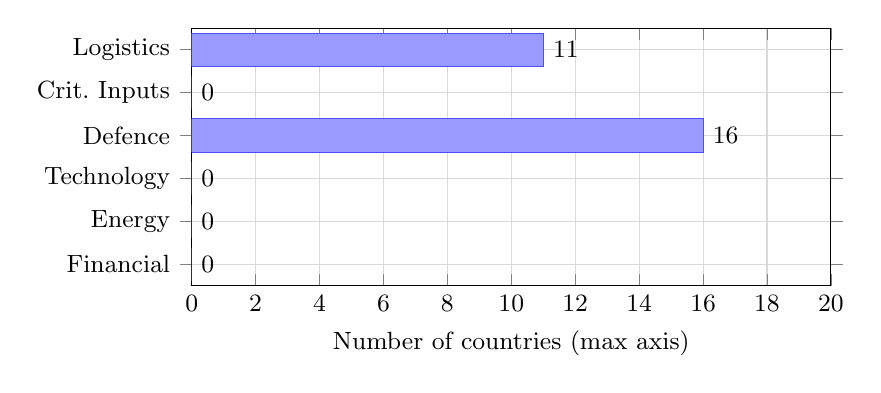
\begin{tikzpicture}
\begin{axis}[
  xbar,
  width=0.80\textwidth,
  height=0.40\textwidth,
  xlabel={Number of countries (max axis)},
  xmin=0, xmax=20,
  ytick={1,2,3,4,5,6},
  yticklabels={Financial, Energy, Technology, Defence, Crit.~Inputs, Logistics},
  y tick label style={font=\small},
  tick label style={font=\small},
  label style={font=\small},
  nodes near coords,
  nodes near coords style={font=\small},
  grid=major,
  grid style={gray!30},
  bar width=12pt,
]
\addplot[fill=blue!40, draw=blue!70] coordinates {
  (0,1)
  (0,2)
  (0,3)
  (16,4)
  (0,5)
  (11,6)
};
\end{axis}
\end{tikzpicture}

\caption{Axis dominance bar chart: count of countries for which each
  axis records the highest score.}
\label{fig:axis-dominance-bar}
\end{figure}

\subsection{Variance contribution decomposition}\label{sec:variance-decomp}

\subsubsection{Formal derivation}

Because the ISI composite is a linear function of six axes
(\cref{eq:composite}), its population variance can be exactly
decomposed via the covariance structure.  We state and prove this
formally.

\begin{quote}
\textbf{Proposition 1} (Variance decomposition of the ISI composite).
\textit{Let $\mathrm{ISI}_i = (1/6)\sum_{j=1}^{6} A_{j,i}$ where
$A_{j,i} \in [0,1]$.  Then}
\begin{equation}\label{eq:var-decomp}
  \operatorname{Var}(\mathrm{ISI})
  = \frac{1}{36}\sum_{j=1}^{6}\sum_{k=1}^{6}
    \operatorname{Cov}(A_j, A_k)\,.
\end{equation}
\end{quote}

\begin{quote}
\textit{Proof.}  By the definition of population variance:
\begin{align}
  \operatorname{Var}(\mathrm{ISI})
  &= \operatorname{Var}\!\Bigl(\frac{1}{6}\sum_{j=1}^{6} A_j\Bigr)
   = \frac{1}{36}\operatorname{Var}\!\Bigl(\sum_{j=1}^{6} A_j\Bigr)
   \notag \\
  &= \frac{1}{36}\sum_{j=1}^{6}\sum_{k=1}^{6}
     \operatorname{Cov}(A_j, A_k)\,,
     \label{eq:var-decomp-proof}
\end{align}
where the second equality uses the bilinearity of covariance.
\hfill$\square$
\end{quote}

The marginal contribution of axis~$j$ to composite variance is
therefore:
\begin{equation}\label{eq:marginal-contrib}
  C_j
  = \frac{1}{36}\sum_{k=1}^{6}\operatorname{Cov}(A_j, A_k)
  = \frac{1}{36}\Bigl[\operatorname{Var}(A_j)
    + \sum_{k \neq j}\operatorname{Cov}(A_j, A_k)\Bigr]\,,
\end{equation}
which decomposes into an \emph{own-variance} component
$(1/36)\operatorname{Var}(A_j)$ and a \emph{cross-covariance}
component $(1/36)\sum_{k \neq j}\operatorname{Cov}(A_j, A_k)$.
The percentage contribution of axis~$j$ is $100 \times C_j /
\operatorname{Var}(\mathrm{ISI})$.

\subsubsection{Empirical results}

\Cref{tab:variance-decomp} presents the marginal contributions.

% Table T8: Variance contribution decomposition
\begin{table}[htbp]
\centering
\caption{Variance contribution decomposition of the ISI composite.  Each axis's
marginal contribution equals $(1/36)\sum_{k=1}^{6}\operatorname{Cov}(A_j, A_k)$,
reflecting both own-variance and covariance with other axes.}
\label{tab:variance-decomp}
\small
\setlength{\tabcolsep}{4pt}
\begin{tabular*}{\textwidth}{@{\extracolsep{\fill}}
  l
  S[table-format=1.6,round-precision=6]
  S[table-format=1.6,round-precision=6]
  S[table-format=3.2,round-precision=2]
  @{}}
\toprule
{\textbf{Axis}} & {\textbf{Var (pop.)}} & {\textbf{Marginal Contrib.}} & {\textbf{\% of Comp.\ Var}} \\
\midrule
  Financial       & 0.001390 & 0.000050 &  1.03 \\
  Energy          & 0.002295 & 0.000169 &  3.46 \\
  Technology      & 0.008947 & 0.000255 &  5.23 \\
  Defence         & 0.050922 & 0.001716 & 35.10 \\
  Critical Inputs & 0.014841 & 0.001023 & 20.92 \\
  Logistics       & 0.034748 & 0.001675 & 34.26 \\
\midrule
  Total           & 0.113143 & 0.004889 & 100.00 \\
\bottomrule
\end{tabular*}
\end{table}


The defence axis contributes 35.10\% and the logistics axis 34.26\%
of composite variance, jointly accounting for 69.37\%.  Critical
inputs contributes 20.92\%.  The three remaining axes---technology
(5.23\%), energy (3.46\%), and financial (1.03\%)---collectively
account for only 9.72\%.

\subsubsection{Own-variance vs.\ cross-covariance decomposition}

\Cref{tab:variance-decomp-detail} further decomposes each axis's
marginal contribution into own-variance and cross-covariance
components.

% Table T8b: Detailed own-variance vs covariance decomposition
\begin{table}[htbp]
\centering
\caption{Decomposition of each axis's marginal contribution into own-variance and
cross-covariance components.  Own: $(1/36)\operatorname{Var}(A_j)$.
Cross: $(1/36)\sum_{k \neq j}\operatorname{Cov}(A_j, A_k)$.}
\label{tab:variance-decomp-detail}
\small
\begin{tabular}{@{}l S[table-format=1.8] S[table-format=+1.8] S[table-format=1.8] S[table-format=2.2] S[table-format=+2.2] S[table-format=2.2]@{}}
\toprule
{\textbf{Axis}} & {\textbf{Own Var}} & {\textbf{Cross Cov}} & {\textbf{Marginal}} & {\textbf{\% Own}} & {\textbf{\% Cross}} & {\textbf{\% Total}} \\
\midrule
  Financial & 0.00003861 & +0.00001188 & 0.00005049 & 0.79 & +0.24 & 1.03 \\
  Energy & 0.00006375 & +0.00010519 & 0.00016894 & 1.30 & +2.15 & 3.46 \\
  Technology & 0.00024853 & +0.00000696 & 0.00025549 & 5.08 & +0.14 & 5.23 \\
  Defence & 0.00141449 & +0.00030164 & 0.00171612 & 28.93 & +6.17 & 35.10 \\
  Critical Inputs & 0.00041226 & +0.00061054 & 0.00102280 & 8.43 & +12.49 & 20.92 \\
  Logistics & 0.00096522 & +0.00071000 & 0.00167522 & 19.74 & +14.52 & 34.26 \\
\midrule
  Total & 0.00314286 & +0.00174620 & 0.00488907 & 64.28 & 35.72 & 100.00 \\
\bottomrule
\end{tabular}
\end{table}

Across the six axes, own-variance accounts for 64.28\% of total
composite variance and cross-covariances for 35.72\%.  The
predominance of own-variance confirms that the ISI composite is
primarily driven by the individual dispersions of the six axes rather
than by their mutual associations.  The cross-covariance share is
nevertheless non-negligible, concentrated in the critical
inputs--logistics ($\operatorname{Cov} = 0.0125$) and
energy--technology ($\operatorname{Cov} = 0.0076$) pairs.

The full $6 \times 6$ population covariance matrix is reported in
\cref{tab:cov-matrix} (\cref{app:tables}).

This variance structure has a direct implication: the ISI composite
ranking is predominantly determined by cross-country differences in
defence and logistics concentration.  The financial axis, despite
measuring a conceptually important domain, contributes negligibly to
cross-country differentiation because its dispersion is small (CV
= 0.2519, $\sigma = 0.037$).

\subsection{Axis contribution to rank differentiation}\label{sec:axis-rank}

The variance decomposition measures each axis's contribution to
\emph{composite variance}.  A complementary question is: how much
does each axis contribute to \emph{rank differentiation}?  We address
this through two statistics:

\begin{enumerate}[leftmargin=2em]
  \item \textbf{Bivariate $R^2$}: the squared Pearson correlation
    between axis score and composite rank (sign-reversed so that
    higher scores correspond to higher rank numbers), measuring the
    share of rank variance explained by each axis alone.
  \item \textbf{Partial correlation}: the Pearson correlation between
    axis score and rank after partialling out the linear effects of
    all other axes, measuring the axis's \emph{unique} association
    with rank conditional on the remaining five axes.
\end{enumerate}

% Table T14: Axis contribution to rank differentiation
\begin{table}[htbp]
\centering
\caption{Axis contribution to composite rank differentiation.  Bivariate $R^2$:
share of rank variance explained by each axis alone.  Partial $r$: association with
rank after controlling for all other axes.}
\label{tab:axis-rank-contrib}
\begin{tabular}{@{}l S[table-format=+1.4] S[table-format=1.4] S[table-format=+1.4]@{}}
\toprule
{\textbf{Axis}} & {\textbf{Pearson $r$}} & {$\boldsymbol{R^2}$} & {\textbf{Partial $r$}} \\
\midrule
  Financial & +0.1571 & 0.0247 & +0.4206 \\
  Energy & +0.3581 & 0.1283 & +0.5496 \\
  Technology & +0.2529 & 0.0640 & +0.7199 \\
  Defence & +0.6273 & 0.3935 & +0.9399 \\
  Critical Inputs & +0.7480 & 0.5595 & +0.8219 \\
  Logistics & +0.7004 & 0.4905 & +0.8089 \\
\bottomrule
\end{tabular}
\end{table}

\Cref{tab:axis-rank-contrib} presents the results.  The bivariate
$R^2$ values confirm the dominance of critical inputs (0.559),
logistics (0.491), and defence (0.394) in explaining rank variation.
Financial has the lowest bivariate $R^2$ (0.025), consistent with its
near-zero variance contribution.

The partial correlations, however, reveal a different ordering.
After controlling for all other axes, defence has the highest partial
correlation (0.940), followed by critical inputs (0.822) and
logistics (0.809).  Technology, which has a low bivariate $R^2$
(0.064), has a substantial partial correlation (0.720), indicating
that conditional on the other five axes, technology provides
meaningful additional rank differentiation.  Even the financial axis,
whose bivariate $R^2$ is only 0.025, has a partial correlation of
0.421, indicating that it contributes non-trivially to rank
differentiation once the effects of other axes are removed.

This pattern is consistent with the full multiple regression of rank
on all six axes, which yields $R^2 = 0.968$ (adjusted $R^2 = 0.958$),
confirming that the six axes jointly explain virtually all rank
variation.  The gap between the bivariate and partial results implies
that the bivariate $R^2$ underestimates the informational content of
low-dispersion axes because it confounds their direct effect with
their low variance.

\subsection{Defence axis structural analysis}\label{sec:defence-structural}

The defence axis warrants dedicated structural analysis because it is
simultaneously the most variance-contributing axis (35.10\%), the most
frequently dominant axis (16/27), and the axis whose removal causes
the largest rank disruption ($\rho = 0.833$).

\subsubsection{Distributional properties}

% Table T16: Defence axis structural analysis
\begin{table}[htbp]
\centering
\caption{Structural properties of the defence axis distribution, EU-27, 2024.}
\label{tab:defence-structural}
\begin{tabular}{@{}lr@{}}
\toprule
{\textbf{Statistic}} & {\textbf{Value}} \\
\midrule
  Countries where defence is max axis & 16 of 27 (59.3\%) \\
  Countries with score $> 0.80$ & 5 (18.5\%) \\
  Countries with score $= 0.00$ & 1 \\
  Mean (pop.) & 0.57319930 \\
  Median & 0.55148593 \\
  Std.\ dev.\ (pop.) & 0.22565797 \\
  Range & 1.00000000 \\
  IQR & 0.31706270 \\
  Skewness & -0.0062 \\
  Excess kurtosis & -0.0337 \\
  Mean def--2nd gap (def-max) & 0.18366014 \\
  Median def--2nd gap (def-max) & 0.11062552 \\
\bottomrule
\end{tabular}
\end{table}

\Cref{tab:defence-structural} reports the key distributional
statistics.  The defence axis spans the full unit interval, from
Slovakia's score of exactly zero to Malta's score of exactly one.
The population standard deviation (\num{0.22565797}) is nearly six
times that of the financial axis.  Five countries record scores above
0.80: Malta (1.000), Netherlands (0.960), Italy (0.921), Sweden
(0.881), and Bulgaria (0.861).  These five countries alone account for
a substantial share of the axis's variance.

\subsubsection{Oligopsonistic character}

The distribution of defence axis scores exhibits features consistent
with oligopsonistic procurement markets:

\begin{enumerate}[leftmargin=2em]
  \item \textbf{Boundary concentration.}  One country scores 1.000
    (Malta), indicating maximal concentration---effectively a single
    dominant supplier.  Five countries score above 0.80, indicating
    very high supplier concentration.

  \item \textbf{Zero outlier.}  Slovakia records exactly 0.000,
    the only zero score on any axis for any country.  This reflects
    the absence of bilateral supplier entries in the SIPRI
    arms-transfer database for Slovakia under the v1.0 methodology,
    not the absence of defence imports.

  \item \textbf{High mean.}  The axis mean (0.573) substantially
    exceeds the financial (0.148), energy (0.365), technology (0.211),
    and critical inputs (0.252) means.  The majority of EU countries
    have concentrated defence-import partnerships.

  \item \textbf{Wide dispersion.}  The coefficient of variation
    (0.394) and the IQR (\num{0.31706}) indicate substantial
    heterogeneity in defence concentration across the EU-27.
\end{enumerate}

\subsubsection{Defence-to-max gap}

For countries where defence is the dominant axis, the defence score
exceeds the second-highest axis score by an average margin of
\num{0.183660}.  \Cref{tab:defence-gap} reports the country-level
defence scores, dominant axes, and defence-to-max gaps.

% Table T16b: Defence gap per country
\begin{table}[htbp]
\centering
\caption{Defence axis score, max axis identity, and defence-to-max gap per country.}
\label{tab:defence-gap}
\small
\setlength{\tabcolsep}{4pt}
\begin{tabular*}{\textwidth}{@{\extracolsep{\fill}}
  r l
  S[table-format=1.4]
  l
  S[table-format=+1.4]
  @{}}
\toprule
{\textbf{Rk}} & {\textbf{Country}} & {\textbf{Def.\ Score}} & {\textbf{Max Axis}} & {\textbf{Gap}} \\
\midrule
  1 & Malta & 1.0000 & Defence & +0.0000 \\
  2 & Cyprus & 0.7484 & Logistics & -0.1925 \\
  3 & Ireland & 0.4488 & Logistics & -0.1648 \\
  4 & Denmark & 0.7236 & Defence & +0.0813 \\
  5 & Croatia & 0.7464 & Defence & +0.2225 \\
  6 & Finland & 0.3896 & Logistics & -0.4076 \\
  7 & Sweden & 0.8810 & Defence & +0.1259 \\
  8 & Austria & 0.5850 & Defence & +0.0591 \\
  9 & Italy & 0.9205 & Defence & +0.4427 \\
  10 & Slovenia & 0.6666 & Defence & +0.2194 \\
  11 & Greece & 0.5514 & Logistics & -0.1683 \\
  12 & Luxembourg & 0.6448 & Defence & +0.0262 \\
  13 & Estonia & 0.3556 & Logistics & -0.1142 \\
  14 & Bulgaria & 0.8606 & Defence & +0.4977 \\
  15 & Netherlands & 0.9595 & Defence & +0.6046 \\
  16 & Hungary & 0.5447 & Defence & +0.0789 \\
  17 & Portugal & 0.4337 & Logistics & -0.0740 \\
  18 & Romania & 0.5635 & Defence & +0.1580 \\
  19 & Czechia & 0.4841 & Logistics & -0.0453 \\
  20 & Poland & 0.4432 & Logistics & -0.0453 \\
  21 & Belgium & 0.4473 & Defence & +0.0952 \\
  22 & Germany & 0.5826 & Defence & +0.2535 \\
  23 & Lithuania & 0.4022 & Defence & +0.0553 \\
  24 & Spain & 0.3808 & Logistics & -0.0514 \\
  25 & Latvia & 0.3407 & Logistics & -0.0274 \\
  26 & Slovakia & 0.0000 & Logistics & -0.4855 \\
  27 & France & 0.3703 & Defence & +0.0174 \\
\bottomrule
\end{tabular*}
\end{table}


The largest gaps are observed for the Netherlands (defence $= 0.960$,
second axis $= 0.355$, gap $= 0.605$) and Bulgaria (defence $=
0.861$, gap $= 0.498$).  These countries' composite rankings are
highly dependent on the defence axis, which explains their sensitivity
to defence-axis removal in the LOO exercise (\cref{sec:loo}).
